\documentclass[tikz]{standalone}
% Common TikZ styles (built from the user's Graduate Macro Sequence template)
\usepackage{tikz}
\usetikzlibrary{arrows.meta, positioning, calc, decorations.markings}

% Base template styles (user-provided)
\tikzset{
  node style/.style={draw, circle, minimum size=6mm, inner sep=0pt},
  label style/.style={font=\small, sloped, anchor=center},
  arrow style/.style={-{Stealth[length=3mm]}, thick}
}

% Macro-diagram extensions (kept minimal and clean)
\tikzset{
  axis/.style={arrow style},
  curve/.style={thick},
  curve2/.style={thick, dashed},
  helper/.style={thin, dashed},
  dot/.style={circle, fill=black, inner sep=1.2pt},
  lab/.style={font=\small},
  titlelab/.style={font=\small\bfseries},
}

\begin{document}
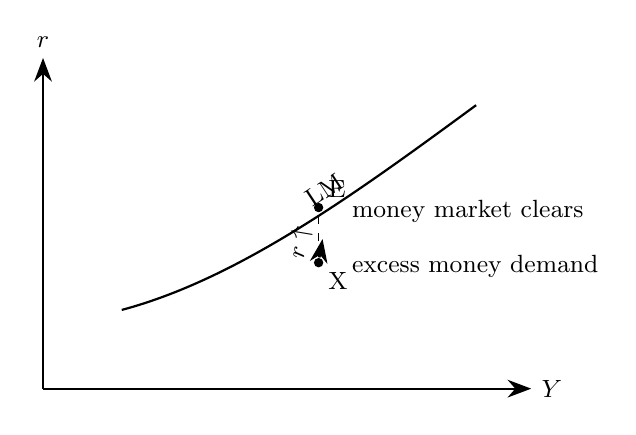
\begin{tikzpicture}[x=1cm,y=1cm]
  \draw[axis] (0,0) -- (6.2,0) node[lab, anchor=west] {$Y$};
  \draw[axis] (0,0) -- (0,4.2) node[lab, anchor=south] {$r$};

  \draw[curve] (1.0,1.0) .. controls (2.5,1.4) and (4.0,2.5) .. (5.5,3.6)
    node[label style, pos=0.60, above] {LM};

  \node[dot] (E) at (3.5,2.3) {};
  \node[lab, anchor=south west] at (E) {E};

  \node[dot] (X) at (3.5,1.6) {};
  \node[lab, anchor=north west] at (X) {X};

  \draw[helper] (X) -- (E);

  \node[lab, anchor=west] at (3.8,1.55) {excess money demand};
  \node[lab, anchor=west] at (3.8,2.25) {money market clears};

  \draw[arrow style] (X) -- (3.55,1.9) node[label style, pos=0.6, above] {$r\uparrow$};

\end{tikzpicture}
\end{document}
